% =========================================================
\section{Semaine 7 : Dérivation Numérique}
% =========================================================

\subsection{Introduction à la dérivation numérique}

\textbf{But :} Approximer $f'(x_0)$ en n'utilisant que des évaluations ponctuelles de $f$.

\textbf{Pourquoi ?}
\begin{itemize}
    \item Expression analytique de $f'$ difficile à calculer.
    \item Expression analytique de $f$ inconnue ($f$ donnée par un algorithme, une "boîte noire").
    \item \textbf{Idée :} Approximation numérique d'équations différentielles.
\end{itemize}

Par définition :
$$f'(x_0) = \lim_{h \to 0} \frac{f(x_0+h)-f(x_0)}{h} = \lim_{h \to 0} \frac{f(x_0)-f(x_0-h)}{h} = \lim_{h \to 0} \frac{f(x_0+h)-f(x_0-h)}{2h}$$

Donc pour $h$ assez petit, une bonne approximation de $f'(x_0)$ devrait être :
\begin{definition}[Formules de différences finies]
\begin{itemize}
    \item $\partial_h^+ f(x_0) := \frac{f(x_0+h)-f(x_0)}{h}$ \quad (formule de différences finies progressives)
    \item $\partial_h^- f(x_0) := \frac{f(x_0)-f(x_0-h)}{h}$ \quad (formule de différences finies rétrogrades)
    \item $\partial_h^c f(x_0) := \frac{f(x_0+h)-f(x_0-h)}{2h}$ \quad (formule de différences finies centrées)
\end{itemize}
\end{definition}

\subsubsection*{Illustration}
\begin{center}
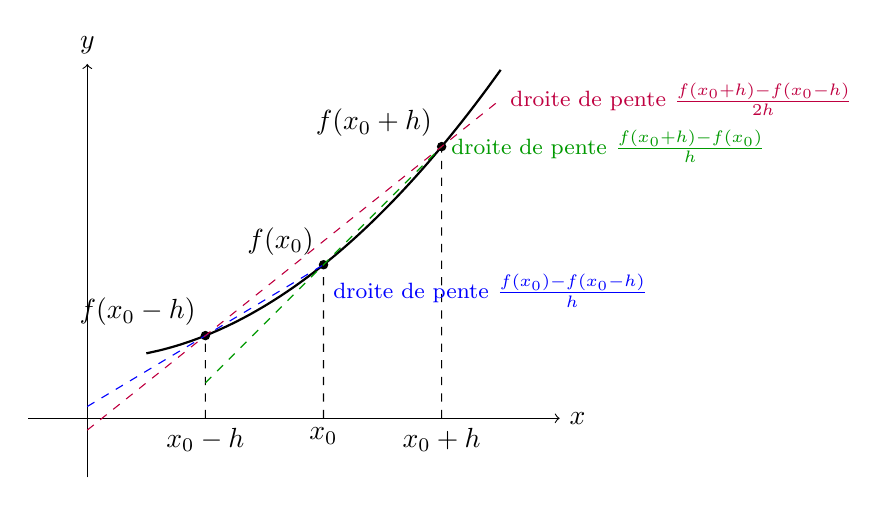
\begin{tikzpicture}[scale=1.5]
    \draw[->] (-0.5,0) -- (4,0) node[right] {$x$};
    \draw[->] (0,-0.5) -- (0,3) node[above] {$y$};
    \draw[thick, domain=0.5:3.5, smooth, variable=\x] plot ({\x}, {0.2*\x*\x + 0.5});
    
    \coordinate (X0) at (2, 1.3);
    \coordinate (XM) at (1, 0.7);
    \coordinate (XP) at (3, 2.3);
    
    \filldraw (X0) circle (1pt) node[above left] {$f(x_0)$};
    \filldraw (XM) circle (1pt) node[above left] {$f(x_0-h)$};
    \filldraw (XP) circle (1pt) node[above left] {$f(x_0+h)$};
    
    \draw[dashed] (1,0) node[below] {$x_0-h$} -- (XM);
    \draw[dashed] (2,0) node[below] {$x_0$} -- (X0);
    \draw[dashed] (3,0) node[below] {$x_0+h$} -- (XP);
    
    \draw[green!60!black, dashed] (1, 0.3) -- (3, 2.3) node[right, font=\footnotesize] {droite de pente $\frac{f(x_0+h)-f(x_0)}{h}$};
    \draw[blue, dashed] (0, 0.1) -- (2, 1.3) node[below right, font=\footnotesize] {droite de pente $\frac{f(x_0)-f(x_0-h)}{h}$};
    \draw[purple, dashed] (0, -0.1) -- (3.5, 2.7) node[right, font=\footnotesize] {droite de pente $\frac{f(x_0+h)-f(x_0-h)}{2h}$};
\end{tikzpicture}
\end{center}

\textbf{Questions :}
\begin{enumerate}
    \item $|f'(x_0) - \partial_h^{+/-} f(x_0)| \to 0$ quand $h \to 0$ ?
    \item Est-ce qu'une des formules est meilleure ?
\end{enumerate}

On observe que $|f'(x_0) - \partial_h^{+/-} f(x_0)| \le Ch$ et $|f'(x_0) - \partial_h^c f(x_0)| \le Ch^2$.

\subsection{Convergence d'une formule de différences finies : exemples}

\begin{proposition}[(1) Preuve pour la formule progressive]
Montrer que si $x_0 \in \mathbb{R}$ et $f \in \mathcal{C}^2([x_0, x_0+h_0])$ pour un $h_0 > 0$, alors :
$$|f'(x_0) - \partial_h^+ f(x_0)| \le Ch$$
avec $C > 0$ indépendante de $h$, $\forall h \le h_0$.
\end{proposition}
\textit{Preuve :} On a par le développement de Taylor :
$$f(x_0+h) = f(x_0) + f'(x_0)h + \frac{f''(\zeta)h^2}{2}, \quad \zeta \in [x_0, x_0+h]$$
Donc :
$$\frac{f(x_0+h)-f(x_0)}{h} = f'(x_0) + \frac{f''(\zeta)h}{2}$$
Ainsi :
$$\left| \frac{f(x_0+h)-f(x_0)}{h} - f'(x_0) \right| = \frac{|f''(\zeta)|}{2}h \le \left( \max_{\zeta \in [x_0, x_0+h_0]} \frac{|f''(\zeta)|}{2} \right) h$$

\begin{proposition}[(2) Preuve pour la formule centrée]
Montrer que si $x_0 \in \mathbb{R}$ et $f \in \mathcal{C}^3([x_0-h_0, x_0+h_0])$ pour un $h_0 > 0$, alors :
$$|f'(x_0) - \partial_h^c f(x_0)| \le Ch^2$$
avec $C > 0$ indépendante de $h$, $\forall h \le h_0$.
\end{proposition}
\textit{Preuve :}
$$f(x_0+h) = f(x_0) + f'(x_0)h + \frac{f''(x_0)h^2}{2} + \frac{f'''(\zeta)h^3}{6}$$
$$f(x_0-h) = f(x_0) - f'(x_0)h + \frac{f''(x_0)h^2}{2} - \frac{f'''(\eta)h^3}{6}$$
Donc :
$$f(x_0+h) - f(x_0-h) = 2h f'(x_0) + \frac{f'''(\zeta)h^3}{6} + \frac{f'''(\eta)h^3}{6}$$
Ainsi, $\forall h \le h_0$ :
$$\left| \frac{f(x_0+h)-f(x_0-h)}{2h} - f'(x_0) \right| \le \max_{\zeta \in [x_0-h_0, x_0+h_0]} |f'''(\zeta)| \frac{h^2}{6} \times 2$$
L'erreur est bien bornée par $Ch^2$.

\subsection{Formules plus générales}

\begin{definition}
Une formule de différences finies qui utilise $m+n+1$ points $x_0+ih$, $i=-m, \dots, 0, \dots, n$ s'écrit :
$$D_h f(x) = \frac{1}{h} \sum_{i=-m}^n \alpha_i f(x_0+ih)$$
avec $\alpha_i$ indépendants de $h$.
\end{definition}

\textbf{Exemple :} La formule de différences finies centrées correspond à $m=n=1$ avec $\alpha_{-1}=-\frac{1}{2}$, $\alpha_0=0$ et $\alpha_1=\frac{1}{2}$ :
$$\partial_h^c f(x_0) = \frac{1}{h}\left(-\frac{1}{2}f(x_0-h)\right) + \frac{1}{h}\left(\frac{1}{2}f(x_0+h)\right) = \frac{f(x_0+h)-f(x_0-h)}{2h}$$

\textbf{Question :} Étant donnés les points $x_0+ih$, $i=-m, \dots, n$, comment choisir les $\alpha_i$ ?
\begin{itemize}
    \item \textbf{Possibilité 1 :} (1) Construire $P$, le polynôme interpolant de degré $(m+n)$ aux points $x_0+ih$. (2) Calculer $P'(x)$. (3) Définir $D_h f(x) := P'(x_0)$.
    \item \textbf{Possibilité 2 (Méthode des coeff. indéterminés) :} On choisit les $\alpha_i$ de sorte à avoir le plus grand ordre possible, i.e., de sorte à annuler le plus de termes possibles dans les développements de Taylor.
\end{itemize}

\subsubsection*{Exemple : Construction avec les développements de Taylor}
$$D_h f(x_0) = \frac{1}{h} \sum_{i=-1}^1 \alpha_i f(x_0+ih) = \frac{\alpha_{-1}}{h}f(x_0-h) + \frac{\alpha_0}{h}f(x_0) + \frac{\alpha_1}{h}f(x_0+h)$$
On peut le ré-écrire avec les développements de Taylor :
\begin{align*}
D_h f(x_0) &= \frac{\alpha_{-1}}{h} \left[ f(x_0) - f'(x_0)h + f''(x_0)\frac{h^2}{2} - f'''(\zeta)\frac{h^3}{6} \right] \\
           &+ \frac{\alpha_0}{h} f(x_0) \\
           &+ \frac{\alpha_1}{h} \left[ f(x_0) + f'(x_0)h + f''(x_0)\frac{h^2}{2} + f'''(\eta)\frac{h^3}{6} \right]
\end{align*}
En regroupant les termes :
\begin{align*}
D_h f(x_0) &= \frac{1}{h} f(x_0)(\alpha_{-1}+\alpha_0+\alpha_1) \\
           &+ f'(x_0)(-\alpha_{-1}+\alpha_1) \\
           &+ \frac{h}{2}(\alpha_{-1}+\alpha_1)f''(x_0) \\
           &+ \frac{h^2}{6}(-\alpha_{-1}f'''(\zeta) + \alpha_1 f'''(\eta))
\end{align*}
Pour approximer $f'(x_0)$, on doit avoir :
$$\begin{cases} \alpha_{-1}+\alpha_0+\alpha_1 = 0 \\ -\alpha_{-1}+\alpha_1 = 1 \end{cases}$$
Pour avoir le plus grand ordre possible, on demande d'annuler le terme d'ordre suivant :
$$\alpha_{-1}+\alpha_1 = 0$$
Le système complet donne :
$$\begin{cases} \alpha_{-1} = -\frac{1}{2} \\ \alpha_0 = 0 \\ \alpha_1 = \frac{1}{2} \end{cases}$$
On retrouve donc la formule de différences finies centrées.

\subsection{Dérivées d'ordre supérieur}
On peut utiliser les mêmes méthodes pour construire une formule $D_h^l f(x_0) = \frac{1}{h^l} \sum_{i=-m}^n \alpha_i f(x_0+ih)$ qui approxime $f^{(l)}(x_0)$.

\textbf{Exemple :} On aimerait construire $D_h^2 f(x) = \frac{1}{h^2}(\alpha_{-1}f(x_0-h) + \alpha_0 f(x_0) + \alpha_1 f(x_0+h))$ pour approximer $f''(x_0)$. On écrit :
$$f(x_0+h) = f(x_0) + f'(x_0)h + f''(x_0)\frac{h^2}{2} + f'''(x_0)\frac{h^3}{6} + f^{IV}(\zeta)\frac{h^4}{24}$$
$$f(x_0-h) = f(x_0) - f'(x_0)h + f''(x_0)\frac{h^2}{2} - f'''(x_0)\frac{h^3}{6} + f^{IV}(\eta)\frac{h^4}{24}$$
Donc :
\begin{align*}
D_h^2 f(x_0) &= \frac{1}{h^2} f(x_0)(\alpha_{-1}+\alpha_0+\alpha_1) \\
             &+ \frac{1}{h} f'(x_0)(-\alpha_{-1}+\alpha_1) \\
             &+ \frac{1}{2} f''(x_0)(\alpha_{-1}+\alpha_1) \\
             &+ h f'''(x_0)\left(\frac{-\alpha_{-1}+\alpha_1}{6}\right) \\
             &+ \frac{h^2}{24}(\alpha_{-1}f^{IV}(\zeta) + \alpha_1 f^{IV}(\eta))
\end{align*}
On doit donc avoir :
$$\begin{cases} \alpha_{-1}+\alpha_0+\alpha_1 = 0 \\ -\alpha_{-1}+\alpha_1 = 0 \\ \frac{\alpha_{-1}+\alpha_1}{2} = 1 \implies \alpha_{-1}+\alpha_1 = 2 \end{cases}$$
Et donc :
$$\begin{cases} \alpha_{-1} = 1 \\ \alpha_0 = -2 \quad \text{\textit{(Note : corrigé par rapport au manuscrit brut)}} \\ \alpha_1 = 1 \end{cases}$$
Finalement :
$$D_h^2 f(x) = \frac{f(x_0+h) - 2f(x_0) + f(x_0-h)}{h^2}$$
En faisant cette construction, on a montré que $|f''(x_0) - D_h^2 f(x_0)| \le Ch^2$, $\forall h \le h_0$ si $f$ était régulière ($\mathcal{C}^4$).

\subsection{Dérivées numériques et erreurs d'arrondis}

Pourquoi est-ce que $|f'(x_0) - \partial_h f(x_0)|$ ré-augmente pour $h$ (très) petit ?
\textbf{Erreur d'arrondis :} L'ordinateur n'évalue pas exactement $f$, mais une approximation $\hat{f}(x) = f(x)(1+\eta)$, avec $\eta \approx 10^{-16}$.

Donc, ce que l'ordinateur calcule est :
$$\hat{\partial}_h^+ f(x_0) = \frac{\hat{f}(x_0+h) - \hat{f}(x_0)}{h} = \frac{f(x_0+h)(1+\eta_1) - f(x_0)(1+\eta_2)}{h} \quad (\eta_1, \eta_2 \approx 10^{-16})$$
$$= \left( \frac{f(x_0+h)-f(x_0)}{h} \right) + \frac{\eta_1}{h}f(x_0+h) - \frac{\eta_2}{h}f(x_0)$$
$$= \left( f'(x_0) + \frac{f''(\zeta)}{2}h \right) + \frac{\eta_1}{h}f(x_0+h) - \frac{\eta_2}{h}f(x_0)$$
Donc :
$$|f'(x_0) - \hat{\partial}_h^+ f(x_0)| \le \max|f''(\zeta)|\frac{h}{2} + 2\max|f(x)|\frac{10^{-16}}{h}$$
L'erreur $\Sigma(h)$ se comporte donc comme :
\begin{remarque}[Erreur totale]
$$\Sigma(h) \approx C_1 h + \frac{C_2 10^{-16}}{h}$$
Une unique minimum en :
$$h_{opt} = \sqrt{\frac{C_2 10^{-16}}{C_1}} \approx 10^{-8}$$
\end{remarque}